% Chinese research note: raw radio geometry, moving attitude acquisition and observability.
% Compile with XeLaTeX in this directory; the comparative figure is generated by synthesize.py.
\documentclass[UTF8,10pt,a4paper,fontset=windows]{ctexart}
\usepackage[margin=21mm,top=18mm,bottom=18mm]{geometry}
\usepackage{amsmath,amssymb,booktabs,graphicx,xcolor,fancyhdr,hyperref}
\definecolor{ink}{HTML}{203B45}
\definecolor{accent}{HTML}{166875}
\hypersetup{colorlinks=true,urlcolor=accent,linkcolor=accent,pdftitle={从航向候选到运动中重启：UWB–IMU定位的模型对照}}
\pagestyle{fancy}\fancyhf{}\fancyhead[L]{\small\color{ink}UWB / IMU \quad 方法札记}
\fancyhead[R]{\small\color{ink}2026 年 11 月}\fancyfoot[C]{\small\thepage}
\setlength{\headheight}{15pt}\setlength{\parindent}{0pt}\setlength{\parskip}{4pt}
\setlength{\abovedisplayskip}{7pt}\setlength{\belowdisplayskip}{7pt}
\newcommand{\parttitle}[1]{\vspace{3pt}{\Large\bfseries\color{accent}#1}\par\vspace{3pt}}
\newcommand{\topic}[1]{\par\smallskip{\bfseries\color{ink}#1}\enspace}
\newcommand{\SO}{\mathrm{SO}(3)}
\newcommand{\Hub}{\rho_{\mathrm H}}
\begin{document}

{\small\color{accent}研究对照 \quad / \quad 测距观测、惯性轨迹与可观性}\par
{\huge\bfseries\color{ink}从航向候选到运动中重启}\par
{\large UWB--IMU 定位的模型对照与适用边界}\par
\medskip
\textbf{核心结果。}同一批实测数据上，端点位置误差的主要来源并不是少求了几个航向极值。先允许惯性轨迹有物理误差，再修正与观测方向有关的无线偏差，能显著降低位置误差。进一步把未知初始姿态直接留在 $\SO$ 上，可以从飞行中的一个短窗估计位置，但不能据此承诺航向交接可靠。

\parttitle{1 \quad 有静止前缀：联合改进两个模型}
基准论文的核心是 $p_i=p_T+\tau_i v_T+R_z(\psi)d_i$，其中 $\tau_i=t_i-T\le0$，$d_i$ 是以端点为基准的二次惯性积分。它用平方测距消元产生航向候选，最终仍在原始 TWR 上拟合。已有 $K=2$ 对照可加自由项 $\tfrac12\tau_i^2c_W$。此次先将它作为强基线。

若常值误差来自机体加计，而机体在旋转，更有物理意义的轨迹为
\begin{equation}
 B_i=\int_{t_i}^{T}(s-t_i)Q(s)\,ds,\qquad
 p_i=p_T+\tau_i v_T+R_z(\psi)[d_i-B_i\,\delta b_a].
\end{equation}
这里 $Q$ 为重力对齐后的名义旋转。项目原有偏置积分；本次的增量是与无线均值联合检验，并拆开两者的贡献。对 $r_i=\|p_i-a\|$、$u_i=(p_i-a)/r_i$，建立
\begin{align}
 \mu_a(r_i,u_i)&=\beta_a+\gamma_a(r_i-\bar r_a)+\kappa_a^\top u_i,\\
 \mathcal L&=\sum_i\Hub\!\left(\frac{r_i+\mu_a(r_i,u_i)-z_i}{\sigma_a}\right)
       +\frac12\|\delta b_a/0.10\|^2 .
\end{align}
$\Hub$ 为阈值 $2$ 的标准 Huber 损失；偏置先验标准差单位为 $\mathrm{m/s^2}$。每锚点系数只用训练日志拟合，正则强度也只在训练日志内选择。$\kappa_a$ 描述经验方向性，不能解释为已辨识的天线误差、锚点测绘偏差或 NLOS 标签。

\begin{center}
{\small\bfseries 表 1 \quad Delft TWR 端点位置误差；单位 m，RMSE / P95}\par
\smallskip\begin{tabular}{lcc}
\toprule 轨迹模型与无线均值 & 全部八锚 & 四个最低锚\\\midrule
仿射 $K=1$，常数均值 & 1.799 / 3.416 & 2.029 / 4.129\\
二次 $K=2$，常数均值 & 0.320 / 0.565 & 0.924 / 1.683\\
旋转偏置，常数均值 & 0.279 / 0.480 & 0.874 / 1.671\\
旋转偏置，距离与方向均值 & \textbf{0.239 / 0.452} & \textbf{0.560 / 1.052}\\
再加同锚时间白化 & 0.249 / 0.470 & 0.535 / 1.014\\\bottomrule
\end{tabular}\end{center}
各方法使用相同 CV 平移种子、四个均匀航向、每起点最多 120 次函数评估。每种布局均为六条后录飞行的 66 个重叠物理窗，六条前录日志用于训练。两布局复用相同时间窗，没有用坐标旋转增样。与强 $K=2$ 相比，第四行 RMSE 降低约 25\% / 39\%；其中无线校准自身在四低锚的六条轨迹均改善，在八锚为四条。

\topic{排除相同动作的训练数据。}每次仅用其余五种动作的前录日志重新选正则强度、拟合无线均值和尺度；各方法共享该五条日志得到的初始化。旋转偏置模型由常数改为几何均值，八锚 RMSE 为 $0.289\to0.250$ m；四低锚为 $0.864\to0.616$ m，六条轨迹均改善。这是同场地跨动作验证，不是跨场地盲测。

\newpage
\parttitle{2 \quad 无静止前缀：把初始姿态留在 $\SO$}
从窗首 $t_0$ 令 $Q(t_0)=I$，只积窗内陀螺角增量。令 $C=R(t_0)$ 为未知初姿、$\ell$ 为已知机体系杆臂。下式将已知世界重力与未知朝向的比力积分分开：
\begin{align}
 F_i&=\int_{t_i}^{T}(s-t_i)Q(s)f_m(s)\,ds,\qquad H_i=F_i+Q(t_i)\ell,\\
 p_{\rm tag}(t_i)&=p_T+\tau_i v_T+\tfrac12\tau_i^2g+C[H_i-B_i\,\delta b_a].
 \label{eq:cold}
\end{align}
$p_T$ 是机体而非天线端点。此处 $B_i$ 按窗首局部 $Q$ 积分。正确陀螺增量、恒定加计偏置及一致的零阶保持离散模型下，该式成立；它不要求启动静止，也不把陀螺漂移建模为常加速度。观察函数可直接切换：
\begin{equation}
 h_{a}(p)=\|p-a\|,\quad
 h_{ab}(p)=\|p-b\|-\|p-a\|,\qquad
 \nabla h_{ab}=u_b-u_a.
\end{equation}
TDoA 是有符号距离差；没有把它平方或伪造成 TWR。本试验逐笔使用记录的异步差分，使用独立标量因子是工作近似，并不证明共享锚点或同步误差相互独立。

\topic{一次姿态起点。}先用纯无线数据拟合带分段加速度先验的轨迹 $\tilde p_i$；它只用于给解算器起点。令 $A=[\mathbf1,\tau]$、$M=I-AA^\dagger$，每行堆叠 $Y_i^\top=(\tilde p_i-\tfrac12\tau_i^2g)^\top$ 与 $H_i^\top$；以初始偏置为零进行种子计算：
\begin{equation}
 (MY)^\top(MH)=U\Sigma V^\top,\qquad
 C_0=U\,\mathrm{diag}(1,1,\det(UV^\top))V^\top .
\end{equation}
最后在原始无线读数上优化式~\eqref{eq:cold}；不把由同一批读数拟合出的 $\tilde p_i$ 再当独立观测。若位置路径精确、无偏置、模型匹配，且 $\mathrm{rank}(MH)\ge2$，两条不共线的已知向量对应唯一的正旋转；秩一时绕该轴的旋转不定。这是对\textbf{已知路径对齐}的充分条件，不是对带噪原始测距的全局恢复证明。

\begin{center}
{\small\bfseries 表 2 \quad 不同输入要求下的 Delft 端点 RMSE（m）}\par
\smallskip\begin{tabular}{lccc}
\toprule 模型 & TWR 八锚 & TWR 四低锚 & TDoA 八锚\\\midrule
纯无线分段加速度平滑 & 0.340 & 0.967 & 0.602\\
静止前缀 + 带先验的常世界加速度修正 & 0.318 & 0.922 & 0.533\\
仅窗内 IMU，全姿态，无附加偏置状态 & \textbf{0.263} & 0.891 & \textbf{0.417}\\
同上，另估有先验的机体加计偏置 & 0.277 & 0.868 & 0.446\\\bottomrule
\end{tabular}\end{center}
表 2 统一采用训练得到的常数无线均值和尺度。Delft 杆臂按零处理，六条 TDoA 测试日志与 TWR 是不同录制；TDoA 使用三条单独训练录制。各格为 66 个窗。第三行四低锚有 8/66 次达到求解上限，仍全部计入；无可用姿态真值，表内只评价位置。八锚 TWR 中第四行的其他单起点得到相近位置，不能把全部位置收益归于 SVD 种子。

\topic{强激励是条件。}四种初始倾角、两种锚高几何、十个配对种子组成的强激励物理模拟中，单个投影姿态起点与 24 起点各有 80/80 个配置低于 $10^\circ$；单位阵起点为 38/80，陀螺补偿后的重力起点为 42/80。弱激励时，投影起点及 24 起点均仅 8/80。这些是模拟配置，不能当作独立实飞成功率。

\newpage
\parttitle{3 \quad 位置可用，不等于航向可交接}
\begin{center}
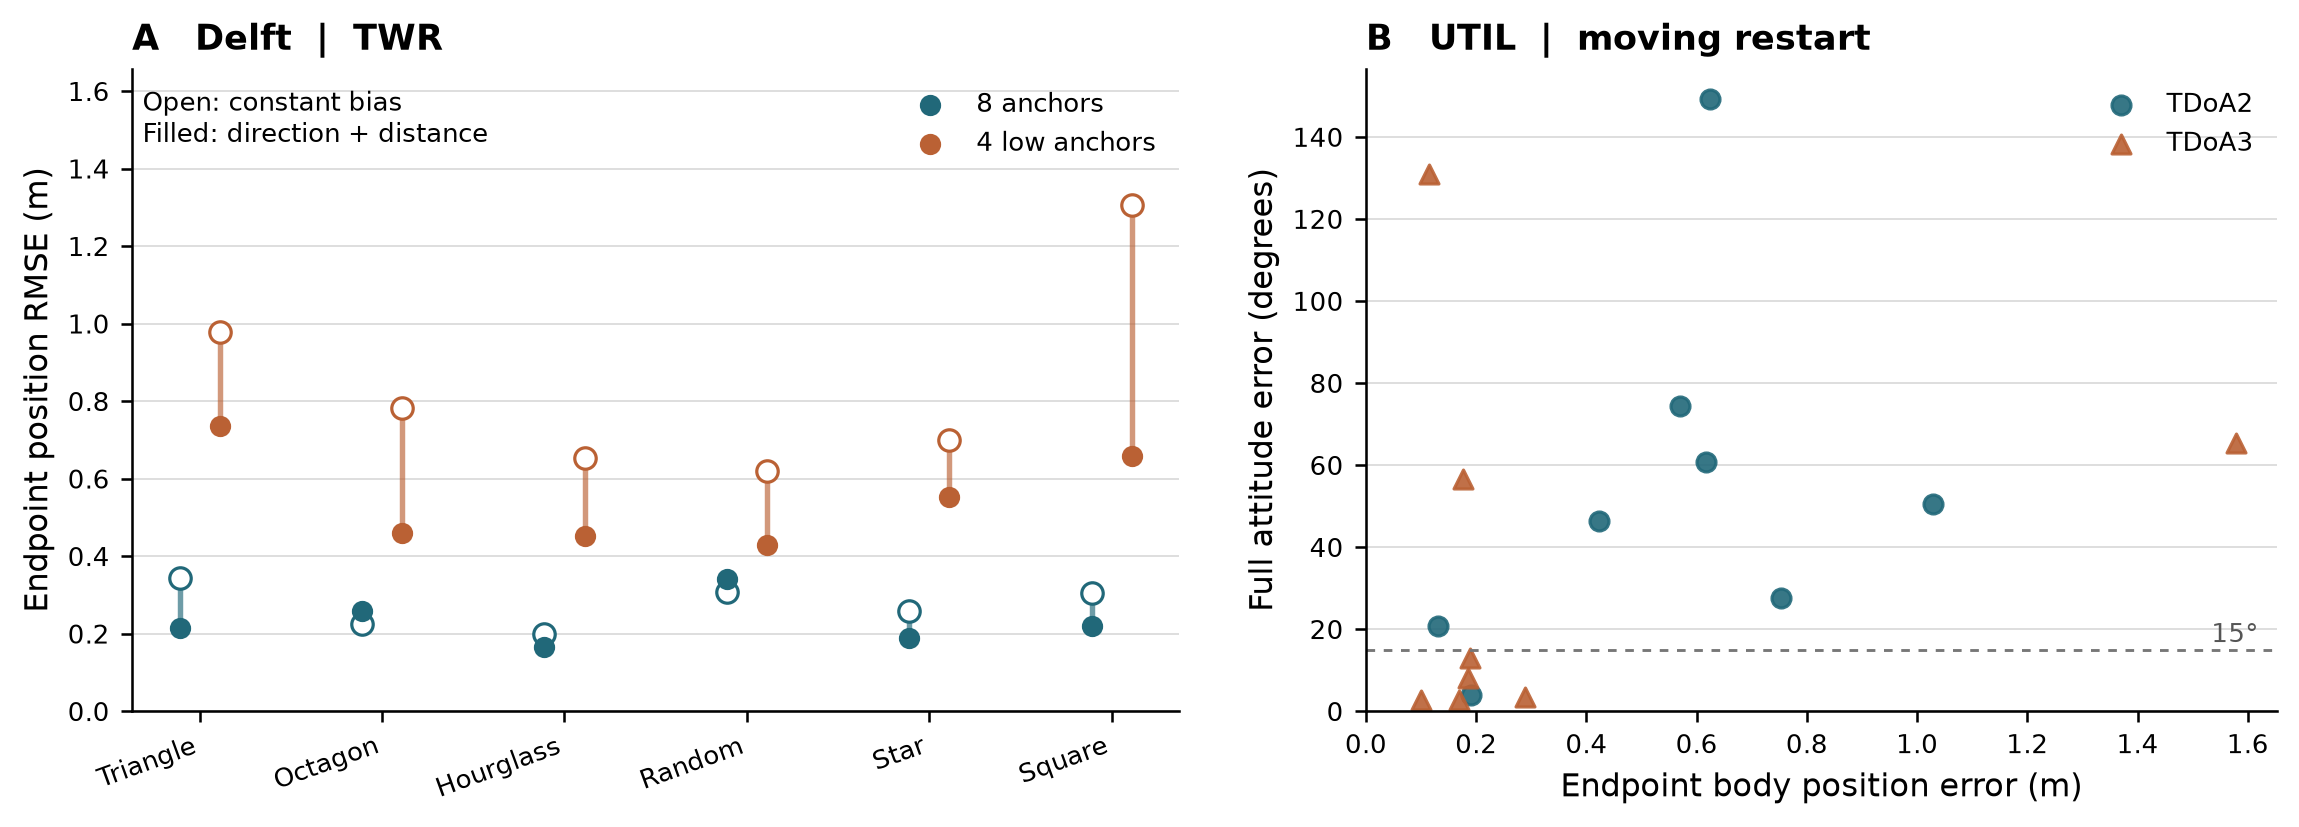
\includegraphics[width=\linewidth]{range_inertial_model_comparison.png}

{\small 图 1 \quad 左：同一惯性模型、同一日志的固定均值与几何均值对照。右：另一个场地中每个窗的机体端点与完整姿态误差；虚线是描述性阈值。}
\end{center}
\topic{跨场地复核。}UTIL 的四种锚点几何与 TDoA2/3 共八条 trial3 录制。每条预定 $[10,16]$、$[25,31]$ s 两个动态窗，真实杆臂进入模型，不用窗前姿态，不对真值做事后配准。含偏置先验的投影起点法，16 个窗的机体位置误差中位数为 0.240 m，完整姿态角误差中位数为 $37.0^\circ$，只有 6/16 低于 $15^\circ$。四均匀起点为 $34.0^\circ$，同样 6/16。不能因代价更低或端点更准就给 InEKF 一个高置信航向。纯无线估计的是天线，未与机体位置直接作优劣比较。

\topic{局部诊断。}设加权原始观测雅可比为 $[J_n,J_R]$，$J_n$ 含平移、速度及自由偏置列。姿态的条件曲率为
\begin{equation}
 \mathcal I_{R\mid n}=J_R^\top(I-J_nJ_n^\dagger)J_R.
\end{equation}
在上述 UTIL 窗里，去掉偏置先验后的最小特征值仅 $0.003$--$0.265~\mathrm{rad}^{-2}$。测距支持弱的方向，应区分由数据约束和由先验决定的部分。此量不是全局多峰检验，也不是已校准的置信概率。

\topic{断距的独立消融。}Delft 六条日志删除 $[15,25)$ s 的无线观测。Profile-1 原策略恢复后等待 2 s 重捕获；单独让在途 InEKF 立即用恢复的测距输出，窗口结束后仍用相同 Profile-1 交接，则恢复后各日志 RMSE 的中位数 $2.197\to0.576$ m，全日志最大误差 $27.715\to17.584$ m，稳定恢复均为 5/6。两种策略在无测距的十秒内逐点相同：这项收益来自恢复后的输出策略。保留完整 15 维先验再优化为 0.573 m，不能证明额外复杂度有独立价值。

\topic{校准迁移边界。}把 TWR 学出的方向误差直接解释成共用锚点位置，在不做目标 TDoA 零偏校准时，八锚全姿态位置 RMSE 由 0.666 恶化到 3.085 m。故训练均值不应作为跨协议的真实测绘修正。同场地 TWR 的窗口收益也不等于整段实时导航提升。

\topic{文献与本试验的关系。}{\small
Jiang 等，ICRA 2024，\emph{Robust Indoor Localization with Ranging--IMU Fusion}：原始测距与惯性因子联合初始化的系统参照（\href{https://doi.org/10.1109/ICRA57147.2024.10611274}{DOI}）。
Zhao、Panerati、Schoellig，RA-L 2021，\emph{Learning-Based Bias Correction for TDOA UWB Localization of Resource-Constrained Mobile Robots}：支持检验位姿相关的无线偏差（\href{https://doi.org/10.1109/LRA.2020.3043199}{DOI}）。Goudar 等，RA-L 2024，\emph{Optimal Initialization Strategies for Range-Only Trajectory Estimation}：用于区分放松问题最优与实际轨迹精度（\href{https://doi.org/10.1109/LRA.2024.3354623}{DOI}）。未声称在本数据上复现并击败这些完整系统。}
\newpage
% Keep the final audit on one page without reducing the body font size.
\begingroup\setlength{\parskip}{2pt}
\parttitle{4 \quad 同窗核查：物理模型收益与候选收益分开}
{\small\color{accent}2026 年 11 月 12 日补充；保留原有试验，新增原稿与当前模型的直接配对。}\par

\topic{同一物理窗，确有水平位置收益。}Delft 六条后录日志的 66 个时间窗、两种布局，共 132 个配置；固定重力对齐 IMU 坐标为 $0^\circ$。原稿缓存与新分支的时间、IMU、逐笔测距、锚点、预积分和真值数组逐项一致；静态无线均值、尺度及六条训练日志也一致。实际端点时间差不超过 $3.6\!\times\!10^{-15}$ s。原稿 Profile-1 与 Uniform-4 的归档三维误差分别复现至 $5.7\!\times\!10^{-7}$、$8.7\!\times\!10^{-8}$ m。

\begin{center}
{\small\bfseries 表 3 \quad 同窗端点 RMSE（m）；XY 为水平范数，Z 为垂向绝对误差}\par
\smallskip{\small\setlength{\tabcolsep}{6pt}
\begin{tabular}{lrrrrrr}
\toprule & \multicolumn{3}{c}{全部八锚，66 窗} & \multicolumn{3}{c}{四个最低锚，66 窗}\\
\cmidrule(lr){2-4}\cmidrule(lr){5-7}
模型 / 起点策略 & XY & Z & 3D & XY & Z & 3D\\\midrule
原稿仿射 / Profile-1 & 1.624 & .756 & 1.792 & 1.665 & 1.169 & 2.034\\
原稿仿射 / Uniform-4 & 1.631 & .760 & 1.799 & 1.665 & 1.159 & 2.029\\
$K=2$ + 几何均值 / 四起点 & .111 & .250 & .273 & .188 & .560 & .591\\
旋转偏置 + 几何均值 / 四起点 & .116 & .209 & .239 & .192 & .526 & .560\\\bottomrule
\end{tabular}}\end{center}

相对原稿 Profile-1，旋转偏置与几何均值组合的 XY / Z / 3D 总体 RMSE 为 $1.645\to.159$、$.984\to.400$、$1.917\to.431$ m；XY 胜 $110/132$，三维胜 $111/132$，六条日志各自的三项 RMSE 均改善。增益被长窗放大：2 / 4 / 8 s 的 XY RMSE 分别为 $.222\to.164$、$.709\to.175$、$3.031\to.126$ m，水平配对胜数为 $37/48$、$37/48$、$36/36$。但相对 $K=2$ 与相同几何均值，XY 总体由 $.1545$ 微升至 $.1590$ m，仅三条日志改善；三维为四条改善。不能宣称旋转偏置全面优于自由二次修正，也不能把组合收益只归于偏置状态。

四个等价坐标下均用同一 Profile-1 候选与相同 CV 初猜，旧模型到新模型的 XY RMSE 为 $1.62498\to.15898$ m，Z 为 $.98148\to.40025$ m，3D 为 $1.89838\to.43067$ m；XY 在 $440/528$ 个配置改善，含 CV 总 nfev 为 $32\,632\to32\,789$（增加 $0.48\%$，不是耗时增幅）。

排除相同动作的训练日志后，组合的 XY / Z / 3D RMSE 为 $.164/.441/.470$ m；相对同样五动作校准的常数均值，XY 胜 $88/132$，三维胜 $98/132$。仅四条日志水平 RMSE 改善，三维为六条。这支持同场地跨动作适配，不构成跨场地无线校准证明。

\topic{固定新目标后，候选只带来较小的优化收益。}冻结旋转偏置、几何均值、先验与停止准则，三臂只改航向种子：Local 为坐标零航向，Profile-1 为原稿放松候选，Uniform-4 为四均匀航向。实际求解 $0^\circ/90^\circ/180^\circ/270^\circ$ 的等价参数化，累计结果为：

\begin{center}
{\small\setlength{\tabcolsep}{9pt}\begin{tabular}{lrrr}
\toprule 策略 & 目标遗漏 / 528 & 含 CV 总 nfev & 三维 RMSE（m）\\\midrule
Local & 7 & 36\,313 & .42856\\
Profile-1 & 0 & 32\,789 & .43067\\
Uniform-4 & 0 & 86\,508 & .43073\\\bottomrule
\end{tabular}}\end{center}

遗漏定义为 $J-J_{\rm best}>10^{-4}(1+J_{\rm best})$，不是全局最优证书。Local 四帧遗漏数为 $0/1/6/0$；Profile-1 的优势是本面板中减少目标遗漏与工作量，不是更低的总体位置误差。三臂原始解算触及 120 次上限的次数为 $3/4/12$，选中解未收敛数为 $3/4/0$，均保留计分。坐标旋转未增加独立实飞样本；nfev 也不代表等量耗时，未作跨机器时延比较。

\topic{QDrone：只检验有限外场适配。}四类场地 10 条录制，按 IMU/TWR 共同支持区间中点取 2 / 4 / 8 s 窗，共 30 窗、10 个端点。棱镜代理 XY RMSE：Profile-1 为 $2.930$ m，四起点仿射为 $2.844$ m，$K=2$ 为 $1.677$ m，旋转偏置为 $1.631$ m。同一旋转偏置目标的 Local / Profile-1 / 四起点各 30 窗：遗漏 $1/0/0$，总 nfev 为 $1677/1429/4174$，Profile-1 的 XY 亦为 $1.631$ m；属评估原四臂后的补验，非独立盲测。相对四起点仿射，2 s 为 $1.634\to1.659$ m，未改善；8 s 为 $4.312\to1.605$ m。发布棱镜已插值；缺少精确 IMU--天线--棱镜外参、原始全站仪时间戳和姿态真值；共同前缀初始化，不作真值配准。无线均值为零、尺度 $.30$ m，未迁移 Delft 系数。故只支持轨迹形状适配，不是精确机体定位或完整几何无线模型的跨场地验证。尚无通用航向交接、恢复新后端或整段 InEKF 收益保证。
\endgroup
\end{document}
